\documentclass[a4paper, 12pt]{extarticle}
\usepackage{graphicx}
\graphicspath{{images/}}
\usepackage{amsmath}
\usepackage{titlesec}
\titlelabel{\thetitle.\quad}
\usepackage{color}
\usepackage{caption}
\usepackage{subcaption}
\usepackage{parskip}
\usepackage{helvet}
\usepackage{hyperref}
\usepackage[T1]{fontenc}

\begin{document}\fontfamily{ptm}
\fontdimen2\font=0.4em

\begin{titlepage}

  \newcommand{\HRule}{\rule{\linewidth}{0.5mm}} % Defines a new command for the horizontal lines, change thickness here

  \center % Center everything on the page

%	HEADING SECTION

  %\textsc{\LARGE University Name}\\[1.5cm] % Name of your university/college
  \text{\Large UNIVERSITY OF SCIENCE AND TECHNOLOGY OF HANOI}\\[0.3cm] % Major heading such as course name
  \textsc{\bfseries UNDERGRADUATE SCHOOL}\\[1.2cm] % Minor heading such as course title
  
\includegraphics[scale = 0.1]{usth.png}\\[1cm]
  \text{ \large Research and Development}\\[0.5cm]
    {\LARGE \bfseries BACHELOR THESIS}  \\ [1cm]
    \text{\large By}\\[0.3cm]
  \text{ \large Bui Vu Huy}\\[0.3cm]
  \text{ \large USTHBI7-082}\\[0.3cm]
  \text{\large Information and Communication Technology }\\[0.5cm]
  
  %	TITLE SECTION
  
  \vspace{1 cm}
  \HRule\\[0.5cm]

  \textbf{\fontsize{18}{20} \bfseries Virtual World Development using Unity Engine}\\[0.3cm] % Title of your document
    \HRule\\[0.5cm]

  
  %	AUTHOR SECTION
  
  \text{\large Supervisor:    Dr. Nguyen Hoang Ha}\\
  
  %	DATE SECTION
  
  \vspace{2.5 cm}
  \textbf{\large Hanoi, \today}\\[3cm] % Date, change the \today to a set date if you want to be precise
  
  
  \vfill % Fill the rest of the page with whitespace
  
\end{titlepage}
\newpage
\part*{\Large Table of Contents}

\newpage

\newpage
\section*{\color{cyan}\Large Acknowledgements}

First of all, i would like to thanks Dr.Nguyen Hoang Ha for giving me 3 months for using the Unity Engine to develop the Virtual World. Also, thank you for supporting me during this internship. 

I also thanks for the USTH ICT Lab for giving me a opportunities to work in a places like in a professional company. 

Finally, I'd like to give special thanks to the guys, girls who made free 3d models, characters in the Unity assets store, so that i can download, use them for my project.
\newpage
 
 \newpage
 \appendix
  \renewcommand{\thesubsection}{\Alph{section}}
 \renewcommand{\thesubsection}{\arabic{subsection}}
\section{\Large Introduction} 
Nowsadays, the technology is getting better and better, so the human life are becoming more and more convenient. With that, people's entertainment needs are also increasing. However, to satisfy people's needs, also to keep up with this rapid development of technology, a virtual world is also a type of entertainment that can satisfy people's need. \\[0.35cm]  A virtual world is a computer-base environment that the user can interact with each other in the world. In general, the virtual world usually using 3-dimensional graphic, with 3D models, which can make people feel like they're in the real world. Virtual worlds allow for multi user to communicate, and a 3D video single player game like Elder Scroll: Blade and Skyrim can still be consider as the virtual world. \\[0.35cm] In general term, there's still no generally accepted definition for virtual world, it supports varying degrees of play and gaming. These are some uses of term: MMOGs game: large number of players within a game, and RPG game, etc... \\[0.35cm] To create a virtual world, there're some types of engine that allow you to make like Unity, Unreal Engine, blender, etc... \\[0.35cm] From one of those engines, Unity is the most popular choice for many people, from beginner to expert. \\[0.35cm] Unity is a cross-platform game engine developed by Unity Technologies, first announced and released in June 2005 at Apple Inc.'s Worldwide Developers Conference as a Mac OS X-exclusive game engine. As of 2018, the engine had been extended to support more than 25 platforms. The engine can be used to create three-dimensional, two-dimensional, virtual reality, and augmented reality games, as well as simulations and other experiences. \\[0.35cm]
 In my opinion, first of all, it has tons of online tutorials to be found, the document with clean format, so a good step for beginners. With it's very intuitive design, C\# language make it easier to use or learn, like you can call other script within a script. Also, with great community, when you have a problem, they'll have you everywhere and every time. Unity has clean API, which is easy to use, understand, implement in C\# code, the application works very well on windows, Linux, android or iOS. Lastly, unlike other engines, the unity has asset store with lots of free assets for everyone to use, while the other ones only have few free assets. \\[0.35cm]In this work, i'll focus on creating the virtual world using unity engine, in particular, it's an RPG game, where you as a player can walk around, interact with other NPC model in the world, or attack some enemy that get in your way. 
  

 To create the virtual world with Unity, first, we'll need to create the terrain by the tools Unity provides for us. After that, we can create my own model and then just simply drag and drop the model into the scene, if not, there're several websites i can get free 3d model from like turbosquid or free3d. For the Lighting and the shadow, Unity also has build-in tool just like other engines, which can help me create the light and shadow easily, adjust it as i want. Furthermore, to make things look good, we can apply some textures to all the objects, prefabs. We can find the texture on google, choose the suitable one for a specific object, and then just simply drag and drop them on that object, or making our own texture. Finally, in order to move around or interact with the object, a camera and player controller should be added into the scene, however, Unity already has the FPScontroller prefab which can be found in the standard assets, we can use it directly without doing anything, but it's still possible to create the character controller from scratch with C\# code.
 \section{\Large Objective} 
 	In this project, since it's about building an RPG game, which is also a type of virtual world, I'll only focus on how to make the player move around the world, is able to interact with other objects around him. In this game, there may be some enemies that get in the way, the player should eliminate them which hurt the player. 
 \section{\Large Aim} 
 	The aim is not necessarily on destroying the enemies, but focus on completing 
 	the quest that villagers in the village gave the player. When finishing a quest, the player should return back to the village, talk to the villagers that you're finished. Beside that, the game should also have an online chat tab , which you can chat with other players who are connecting to the same network while playing game, they may help you finishing the quest faster. 

 
 \newpage
 \setcounter{secnumdepth}{4}
 \titleformat{\paragraph}
 {\normalfont\normalsize\bfseries}{\theparagraph}{1em}{}
 \titlespacing*{\paragraph}
 {0pt}{1.25ex plus 1ex minus .2ex}{1.5ex plus .2ex}
 
  \section{\Large Programs, Materials and Methods}
  	\subsection{External programs used}
  		\subsubsection{3DS Max}
 		 3DS Max, a program developed by Autodesk, previously called 3D Studio Max, is a 3D computer graphics program for making 3D animations, models , images...
 		 This program was used in this project in order to edit UV mapping of some models, correct the position of the texture. 
 		 \subsubsection{Photoshop}
 		 Photoshop is a photo editing and graphic design software. It is developed by Adobe Systems for MacOS and Windows. It's not like other graphic design or photo editing softwares, it can create normal map, height map, occulusion map from a single texture. With this, this software will help me with the technique bump mapping, so the game's texture will look more realistic. 
 		 \subsubsection{Visual Studio}
 		 Visual studio is an IDE (integrated development environment ) from Microsoft. It's used to develop computer programs, as well as websites, supports many programming languages such as : C++, C\#, JavaScript, etc... 
 		 This is the main software of this project, because i'm using this one to write scripts in order to make the game works.
 		 When installing unity 5, normally it's shipped with visual studio community which is free for everyone. Previously, it's shipped with the monodevelop, but now the monodevelop is discontinued, no longer support unity, replaced with visual studio community as it's more powerful than monodevelop, it support MacOS and windows, gives you a cloud storage for saving like one drive(when you project goes wrong), which monodevelop doesn't have.  
 		
 		 
 		 
 		 \subsection{Materials}
 		 \subsubsection{DirectX}
 		 DirectX is the collection of API (or  application programming interfaces), also made by Microsoft, for handling task related to multimedia. It contains these APIs such as Direct3D, DirectDraw, DirectMusic, DirectSound .... , especially for game programming. \\[0.15cm] The DirectX version use in this project here is Direct X11 because from unity 4.x or higher, the engine tend to use more cpu cores, and with Direct3D 11, it has improved multi-threading support so it can utilize multi-core better. Without Direct X, the engine cannot simulate the light in the game or even run. 
 		 \subsubsection{A dedicated graphic card}
 		 A graphic card with direct x11 compatible is compulsory for Unity. Because unity comes with MSAA support, to improve image, textures quality, which direct x10 or lower doesn't support. Integrated GPU is fine also as long as it's powerful enough to run unity programs, games and have direct x11 compatible. 
 		 
 		 \subsection{Method}  
 		 \subsubsection{Overview Diagram}
 		 - In this section, i'd like to introduce my overview diagram about the concept of creating a virtual world: \\[0.20cm] \par
 		 
 		 	\begin{figure}[h]
 		 		\centering
 		 		\includegraphics[width=0.65\columnwidth]{Overview_diagram.png}
 		 		\captionof{figure}{Overview Diagram}
 		 		\label{fig:Overview1}
 		 	\end{figure}
 		 \newpage
 		 
 		 \newpage
 		  \subsubsection{Details}
 		  \paragraph{Preparation}
 		  Unity can be download from the \href{https://store.unity.com/}{offical website}. I prefer Unity personal version because it's free, for everyone. As i mentioned before, to be able to run Unity, and create a new project, you'll need at least direct x11 for simulate lighting, shadows on the scene. To create a terrain, which is the base of the virtual world, all i have to do is go to game object -> 3D Object -> Terrain. The terrain width and length is only set to 500x500, which i think is big enough for this project.  \begin{figure}[h]
 		  	\centering
 		  	\begin{minipage}{.4\textwidth}
 		  		\centering
 		  		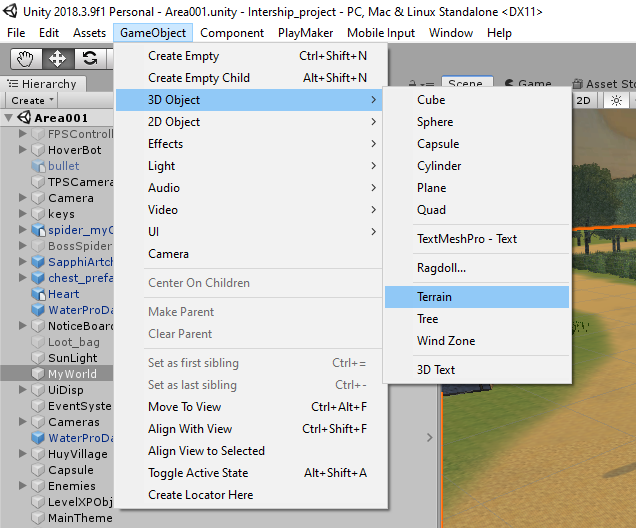
\includegraphics[width=1\linewidth]{intructions/1.png}
 		  		\captionof{figure}{Create terrain}
 		  		\label{fig:test2}
 		  	\end{minipage}
 		  	\begin{minipage}{.4\textwidth}
 		  		\centering
 		  		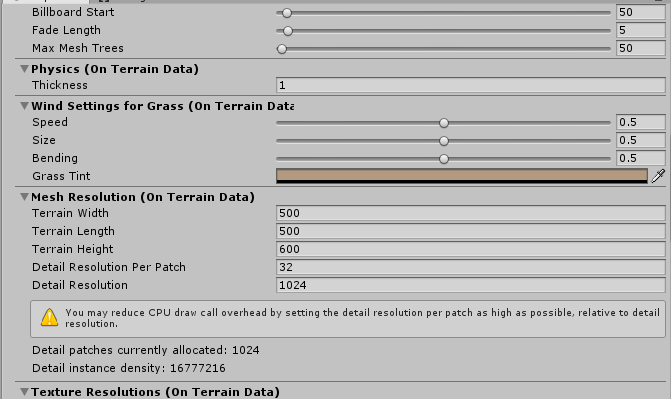
\includegraphics[width=1.4\linewidth]{intructions/2.png}
 		  		\captionof{figure}{Properties}
 		  		\label{fig:test3}
 		  	\end{minipage}
 		  \end{figure}
 	  \\[0.15cm]
 	  From the Inspector section, there're 4 sections: Paint texture, paint trees, paint details. Each of these sections has painting tool with 20 brush presets, resizable brush size, opacity. For the textures, you can use any texture you want for the terrain, for example i use this texture from this website: \href{https://www.textures.com/download/grass0153/48704}{https://www.textures.com/download/grass0153/48704}. The same applied for painting details, but for painting trees, the material for this one is 3D model, however it can be found in the Standard Assets which comes with Unity when installed. 
 	   \begin{figure}[h]
 	   	 \centering
 	   	 \begin{minipage}{1\textwidth}
 	   	 	\centering
 	   	 	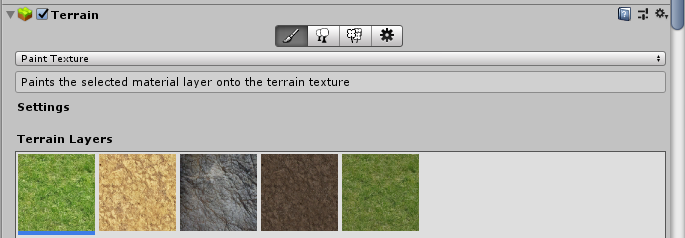
\includegraphics[width=0.75\linewidth]{intructions/3.png}
 	   	 	\captionof{figure}{Sections}
 	   	 	\label{fig:test4}
 	   	 \end{minipage}
 		 \end{figure}  
 		 \newpage
 		 
 	\newpage
 	Besides, to make the terrain looks better, the user can also raise or lower the terrain to create mountains, river. After i finish creating the terrain, all i have to do is drag and drop other objects/prefabs into the scene, put the textures corresponding to each object, while these prefabs/objects can be found on unity assets store or from free3d website as i mentioned from the introduction. 
 	 \paragraph{Player}
 	 To be able to interact with the objects, NPCs, a player should be added into the scene. For example, i use this little robot for my player: \href{https://free3d.com/3d-model/bb8-35865.html}{https://free3d.com/3d-model/bb8-35865.html}. 
 	\newpage
\end{document}